\input format

\usepackage{tikz}
\usepackage{graphicx}
\usepackage{amssymb}
\usepackage{amsmath}
\usepackage{harpoon}
\usepackage{float}
\usepackage{enumerate}
\usepackage{algorithm}
\usepackage{algpseudocode}
\usepackage{subcaption}
\usepackage{bm}
\usepackage{listings}


\usetikzlibrary{fit,positioning}

\begin{document}
\begin{flushleft}

\bf{DD2424 Assignment 1 Report (For Optional Part)} \\
\bf{Zesen Wang} \\


\end{flushleft}



\section{Optimize the Performance of the Network}

In this part, I choose to implement (a), (d) and (e).

For (a), I load all training data, and I use the first 1000 samples as the validation set.

For (d), I use exponential decay, the formula for the decay is 
\[
	\eta = \eta_0 e^{-kt}
\]
where $k$ is a hyperparamter (set to 0.1 in experiment), and $t$ is the number of epoch.

For (e), Xavier initialization is implemented for the initialization of $W$ and $b$. Xavier will stabilize training because it constrains the range of initial parameters, which makes the gradient constrained in a proper interval which is not too large or too small. The stable gradient ensures the stable training.

\begin{verbatim}
Optimization method: (a), (d), (e)
lambda=0, n_epochs=40, n_batch=100, eta_0=0.01
Accuracy on test set: 0.4017
\end{verbatim}

\begin{verbatim}
Optimization method: (a)
lambda=0, n_epochs=40, n_batch=100, eta=0.01
Accuracy on test set: 0.3972
\end{verbatim}

\begin{verbatim}
Optimization method: (d)
lambda=0, n_epochs=40, n_batch=100, eta_0=0.01
Accuracy on test set: 0.3768
\end{verbatim}

\begin{verbatim}
Optimization method: (e)
lambda=0, n_epochs=40, n_batch=100, eta=0.01
Accuracy on test set: 0.3693
\end{verbatim}

\begin{verbatim}
Optimization method: None
lambda=0, n_epochs=40, n_batch=100, eta=0.01
Accuracy on test set: 0.3665
\end{verbatim}

Compared with the experiment with no optimization method applied, the method (a) promotes the accuracy on test set most among three methods. And the combination of them generates the best result which is 0.4017.

\newpage
\section{SVM Multi-class Loss}

\begin{verbatim}
lambda=0, n_epochs=60, n_batch=100, eta=0.001
Accuracy on test set: 0.3576
\end{verbatim}

\begin{figure}[h!]
	\centering
	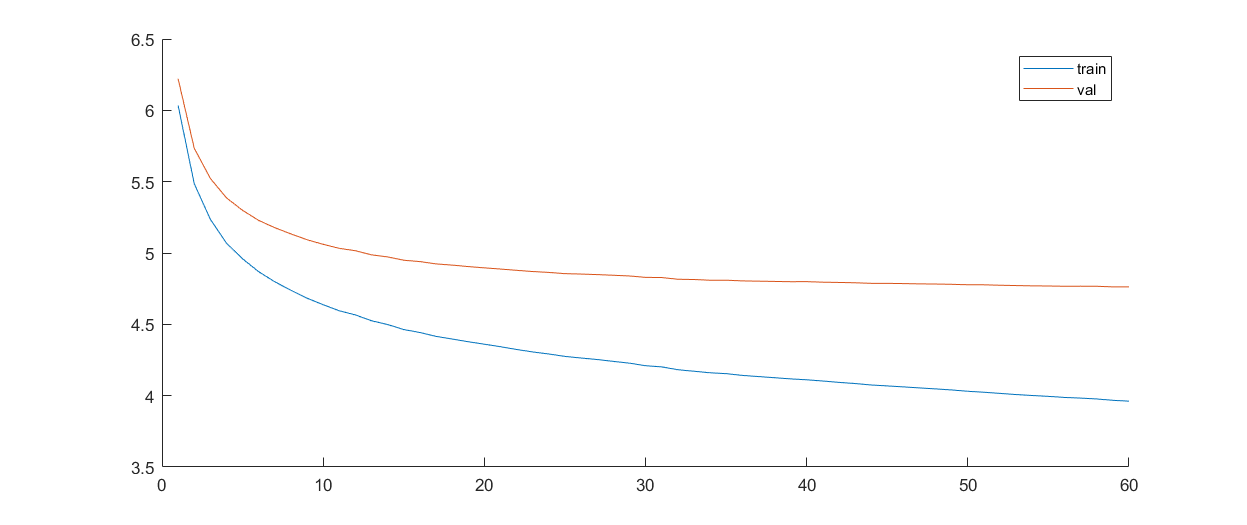
\includegraphics[width=0.65\textwidth]{../Result_Pics/a6.png}
\end{figure}

\begin{verbatim}
lambda=0, n_epochs=60, n_batch=100, eta=0.002
Accuracy on test set: 0.3388
\end{verbatim}

\begin{figure}[h!]
	\centering
	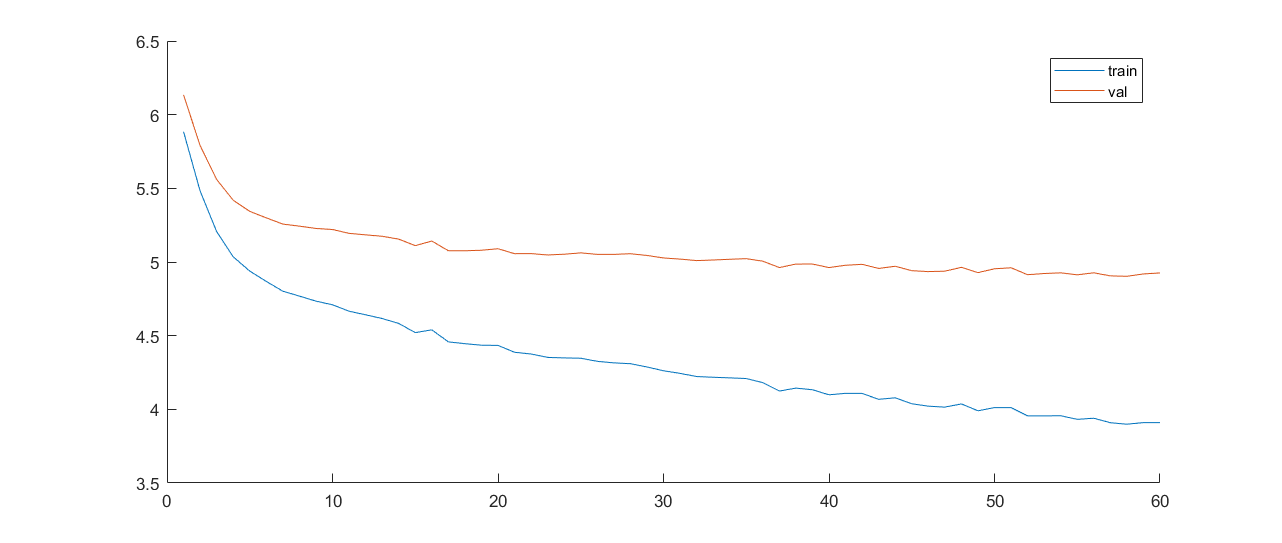
\includegraphics[width=0.65\textwidth]{../Result_Pics/a7.png}
\end{figure}

\begin{verbatim}
lambda=1e-3, n_epochs=60, n_batch=100, eta=0.001
Accuracy on test set: 0.3569
\end{verbatim}

\begin{figure}[h!]
	\centering
	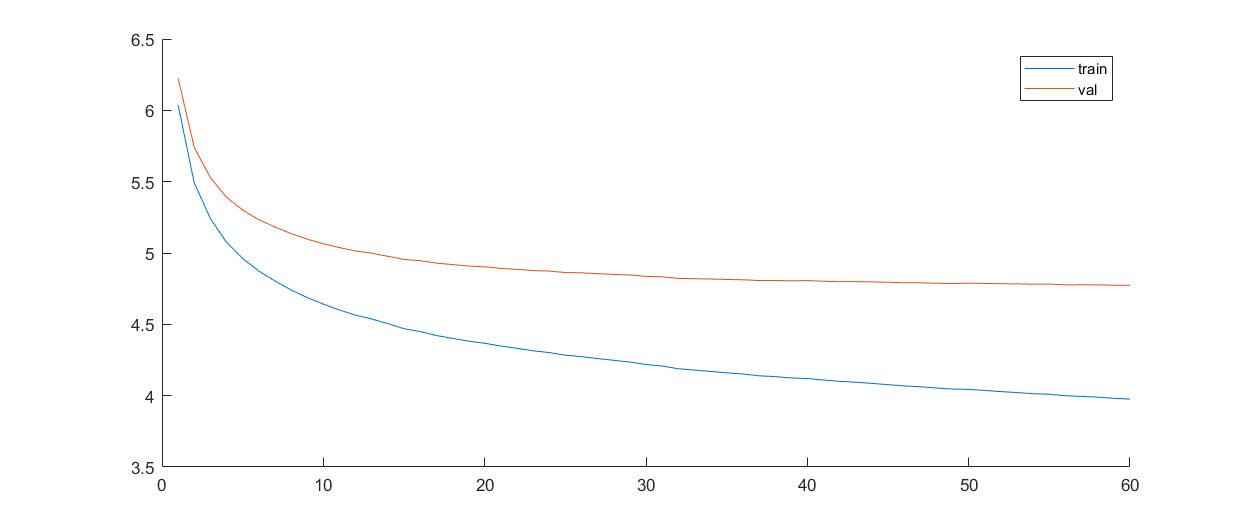
\includegraphics[width=0.65\textwidth]{../Result_Pics/a8.png}
\end{figure}

According the results, the best result it can get it's about 0.36, and in this section, it uses 60 epochs for training. Therefore, the performance with cross-entropy loss is better than the performance with SVM loss.

\end{document}


